\documentclass[11pt]{article}

% ---------- Packages ----------
\usepackage[margin=1in]{geometry}
\usepackage{amsmath,amssymb,amsthm}
\usepackage{booktabs}
\usepackage{graphicx}
\usepackage{hyperref}
\usepackage{xcolor}
\usepackage{listings}
\usepackage{array}
\usepackage{titlesec}
\usepackage{enumitem}
\usepackage[protrusion=true,expansion=false]{microtype}
\usepackage{setspace}
\usepackage[numbers,sort&compress]{natbib}

% ---------- Style ----------
\hypersetup{
  colorlinks=true,
  linkcolor=black,
  citecolor=blue!60!black,
  urlcolor=blue!60!black
}

\titleformat{\section}{\large\bfseries}{\thesection}{0.7em}{}
\titleformat{\subsection}{\normalsize\bfseries}{\thesubsection}{0.6em}{}

\lstdefinestyle{code}{
  basicstyle=\ttfamily\footnotesize,
  breaklines=true,
  frame=single,
  framesep=4pt,
  xleftmargin=6pt,
  xrightmargin=6pt,
  backgroundcolor=\color{gray!6},
  keywordstyle=\color{blue!60!black},
  stringstyle=\color{red!50!black},
  commentstyle=\color{gray!70!black}\itshape,
  showstringspaces=false
}
\lstset{style=code}

\setlength{\parskip}{0.4em}
\setlength{\parindent}{0pt}

% ---------- Title block ----------
\title{\textbf{A Chess Tutor You Don't Want to Punch in the Face}\\
       \large A Level-Aware Chess Coach That Explains Moves Beginners Can Actually Use}
\author{STA 561}
\date{Spring 2026}

\begin{document}

\maketitle

{\Large \textbf{Group Members}}\\[0.3cm]
\begin{tabular}{l}
Member 1: Yuhang Sun \\
Member 2: Jianqi Feng \\
Member 3: Jiaqi Zhang \\
Member 4: Luke Sun \\
Member 5: Zhihan Chen \\
\end{tabular}

% ==========================================================================
\section*{Executive Summary}
\addcontentsline{toc}{section}{Executive Summary}
% ==========================================================================

\subsection*{The problem}
Chess engines like Stockfish can tell you the objectively best move in any position. But ``best'' and ``useful'' are not the same thing for a beginner. A 600-rated player told to play a twelve-move tactical combination learns nothing: the move is correct but incomprehensible. What beginners need is a tutor that recommends moves they can actually understand, execute, and learn from. The assignment brief frames this exact gap, asking for a tutor that ``maximizes a given player's improvement rather than providing the right recommendation if one were playing against an engine.''

\subsection*{Our approach}
We built an interactive tutor that separates two questions: what is the strongest move, and what is the most useful move for this player right now. Every legal move gets several scores. One reflects how strong the move is objectively (using a professional-strength engine when available, and a simpler built-in evaluator when it is not). Another measures how good the move is as a \emph{teaching} move for a player at a particular skill level. Others capture how hard the move is to find, how risky it is, and how likely a real person at that level is to actually play it. When the strongest move and the most teachable move disagree, the tutor explains the trade-off. The system supports four skill levels (rated 600, 1000, 1400, and 1800 in standard chess terms) and three modes: a position analyzer for studying any board you set up, a play-against-bot mode with running commentary and post-game review, and an evaluation dashboard that demonstrates the tutor's behavior across curated test positions.

The new part of the project is that the tutor's recommendations are informed by data from real games, not purely hand-tuned rules. Instead of us deciding how much to reward castling or how much to punish complicated moves, we let real games decide. We used thousands of real online games to learn what players at different levels tend to notice, miss, and understand. The tutor uses that information to recommend moves that are not only strong, but teachable for the selected level.
The first component learns what moves humans at each skill level actually choose. The second learns what real players at a given level value in a move---which factors like complexity, center control, and king safety matter most---so that the tutor's weighting is learned from games rather than hand-picked. The results of both are baked into the tutor and used every time it makes a recommendation. A small, lightweight layer on top of this also watches how the current user is playing during the session and nudges the tutor to be a bit stricter or a bit gentler accordingly.

\subsection*{Results}
The system shows clear skill-dependent behavior: it predicts real player choices substantially better than random guessing, and its learned weighting captures the intended educational pattern that weaker players should be steered away from overly difficult moves while stronger players can stay much closer to engine-best play.

We evaluate the tutor end-to-end on two curated test suites covering 30 position cases and 4 post-game review cases. On the position benchmark, the tutor matches the intended teaching theme 93.3\% of the time and respects skill-level constraints in 86.7\% of cases. When all dimensions must pass simultaneously---including exact keyword matching in explanations---the strict pass rate is 26.7\%, with the keyword criterion as the main bottleneck rather than the quality of the advice itself. On the review benchmark, all four cases pass on weakness detection, actionable next-step generation, and annotation consistency.

The benchmark was designed to stress-test the system across diverse positions, opening types, and skill levels, and the imperfect scores point to concrete areas for improvement. Separately, a blind side-by-side comparison with 1{,}572 evaluations found that the tutor's advice is preferred over raw engine output on clarity (98.9\%), usefulness (87.8\%), and being less overwhelming (96.1\%) across all three tested skill levels.

\subsection*{Future work}
The most important extension is a real user study with novice players, tracking whether time spent with the tutor actually raises their rating. Other valuable extensions: a more realistic simulation of human play so that playing against the 1000-rated bot feels unmistakably different from playing the 1400-rated bot; live import of the student's own games from Lichess or Chess.com so the review mode operates on real play rather than pasted text; and a training setup that shares information across skill levels so our weakest data band (around 600) borrows strength from the better-covered bands.

\newpage

% ==========================================================================
\section*{Frequently Asked Questions}
\addcontentsline{toc}{section}{Frequently Asked Questions}
% ==========================================================================

\subsection*{Q1. Why not just use Stockfish directly?}
Stockfish always recommends the objectively strongest move, which is what a grandmaster needs~\cite{silver2018alphazero}. For a 600-rated beginner, the strongest move is often incomprehensible---imagine asking a first-grader to learn addition from the Peano axioms. Our tutor solves a different problem: picking a move the student can understand and learn from, even if that means sacrificing a few centipawns. Concretely, the tutor score penalizes moves that require deep calculation (high \texttt{difficulty}), rewards moves that address the student's immediate weaknesses such as undeveloped pieces or an exposed king, and rebalances these trade-offs by ELO level. None of that information exists in Stockfish's raw evaluation.

\subsection*{Q2. How were the model parameters learned, and could they be wrong?}
The parameters come from Bayesian inference on real Lichess games. We downloaded roughly 1{,}500 rated games per ELO band using the public Lichess API (no authentication needed for game exports), kept only games where both players fell inside the target rating window, replayed each game position-by-position through the heuristic engine to produce a feature row per candidate move, and labeled the row the human actually picked. We then fit two models in PyMC~\cite{salvatier2016pymc} using the No-U-Turn sampler~\cite{hoffman2014nuts}: a conditional logit model for human move choice (Model A) and a logistic regression for teaching quality (Model B). We confirmed convergence by checking that every R-hat fell below 1.05; bulk ESS ranged from roughly 330 to 1{,}250 for Model~A and 900 to 1{,}400 for Model~B across features and bands.

The Bayesian framework gives more than point estimates: every coefficient has a full posterior distribution, so we know how confident we are in each weight. For example, the \texttt{difficulty} penalty in Model~B has a 94\% HDI of $[-0.24, -0.15]$, which excludes zero and confirms the complexity penalty is real, not an artifact of noise. Conversely, \texttt{num\_priorities} has an HDI spanning zero, signaling low confidence in that weight. Tables~\ref{tab:modelA-selected} and~\ref{tab:modelB-selected} report $\pm$ posterior standard deviation (SD) for every coefficient, and Figure~\ref{fig:posteriors} visualizes the intervals. We also keep the handcrafted heuristic as a graceful fallback, so if the learned parameters are ever missing or produce anomalies the system degrades to the original behavior.

\subsection*{Q3. How do you know the tutor actually helps beginners improve?}
We do not claim a randomized outcome study, so we do not claim to have proven rating improvement directly. What we \emph{do} provide is a layered body of evidence that the tutor behaves more like a teaching system than a raw engine wrapper.

\emph{Prediction accuracy.} Model A predicts actual human move choices substantially better than random guessing across all four bands, which shows that it has learned meaningful human-like move preferences rather than arbitrary weights.

\emph{Behavioral differentiation.} The tutor gives different recommendations at different skill levels in the same position. That is one of the core requirements of the project: the 600-rated player should not be taught in the same way as the 1800-rated player.

\emph{End-to-end benchmark performance.} On a curated 30-position benchmark suite, the tutor matches the intended teaching theme 93.3\% of the time and respects level-fit constraints in 86.7\% of cases. The overall strict pass rate is 26.7\%, with explanation completeness (26.7\%) as the main bottleneck. On the review benchmark, all four cases pass on weakness detection, next-step actionability, and annotation consistency. These imperfect numbers are the honest output of an expanded stress test, not a sign that the system fails to teach---the theme and level-fit rates show that the tutor's core recommendations are sound, while the lower explanation rate points to a specific, improvable weakness in the commentary pipeline.

\emph{Data-driven tutor weights.} Model B replaces hand-tuned scoring weights with coefficients learned from real player behavior, ensuring the tutor's weighting of complexity, positional improvement, and tactical risk reflects what players at the target level actually notice and value rather than what we guessed they would.

\emph{A/B preference evidence.} In a blind study with 1{,}572 LLM-simulated comparisons across three persona levels (600, 1000, 1400), the tutor's advice was preferred over raw engine output on usefulness by 97.9\% at 600, 86.3\% at 1000, and 79.2\% at 1400. Even at the club level the engine was preferred in only 1.0\% of cases; the remainder were ties. This is qualitative, not experimental, evidence---but it directly addresses the project brief's request to show that the system is ``more user friendly than simply using a chess engine.''

So our evidence spans \emph{behavioral validity} (benchmark performance, behavioral differentiation) and \emph{comparative preference} (A/B study). A true learning-outcomes study with real players would be the natural next step.


\subsection*{Q4. Do recommendations really differ between skill levels?}
Yes, substantially, and the mechanism is visible in the learned weights. For Model A (which predicts human move choice), the coefficient on \texttt{num\_preferred\_tags} rises from $-0.15$ at ELO 600 to $+0.36$ at 1400 and $+0.26$ at 1800---stronger players increasingly gravitate toward moves aligned with level-appropriate strategic themes, while beginners do not yet notice these patterns. The \texttt{difficulty} coefficient shows a non-monotonic but interpretable pattern: $-0.36$ at 600, near zero at 1000 ($+0.06$), and strongly negative at 1400 and 1800 ($-0.79$)---intermediate players do not yet systematically avoid complex moves, but club and advanced players do. For Model B (which covers only the 1800 band; see Q8), the learned weights confirm the educational intent: \texttt{difficulty} is $-0.20$ (penalizing complex moves), while \texttt{center\_change} ($+0.17$) and \texttt{king\_safety\_change} ($+0.11$) reward strategic improvements. These are not properties we encoded by hand; they fell out of the data.

\subsection*{Q5. How does the session-level Bayesian adapter interact with the trained models?}
Model A and Model B are trained once, offline, on Lichess data, and their posterior means are baked into a JSON file read at startup. The session adapter is a small second-stage posterior initialized fresh at the beginning of each session. After each user move it receives a signal---for example, the feature delta between the move the user chose and the tutor's recommended move, plus the outcome classification---and performs a diagonal-Gaussian posterior update over a small set of coefficients. It tracks a scalar \texttt{skill\_mean} and \texttt{skill\_variance} with a Kalman-style update, and uses that skill estimate to adjust the session's \texttt{complexity\_weight} and \texttt{max\_eval\_loss}. It never rewrites the trained parameters; it only adds a bounded additive correction. This is intentional---we want global behavior determined by data, with only gentle local personalization on top.

\subsection*{Q6. Why both a Stockfish path and a heuristic path? Isn't that over-engineering?}
The dual path exists for robustness, reproducibility, and pedagogy. For robustness, Stockfish is a separate executable that may be missing, wrong architecture, or blocked on a grader's machine; we want the demo to work regardless. For reproducibility, our feature extraction pipeline \emph{forces} the heuristic mode so that the training CSVs are deterministic; if we trained on Stockfish-derived labels we would make the results depend on the specific engine build. For pedagogy, the heuristic's components---material, piece-square tables, king-ring safety, center control, hanging-piece detection, mobility---correspond one-to-one to the teaching themes the tutor uses in commentary, so when we explain a move to the user in terms of ``king safety'' or ``center control'' we are pointing to a real component of the scoring function rather than a derived concept.

\subsection*{Q7. Why a conditional logit for Model A rather than an ordinary classifier?}
Because the task is a conditional choice over a position-specific feasible set, not a prediction about an individual move in isolation~\cite{mcfadden1974conditional}. A conditional logit with softmax over the legal candidates is the natural statistical object: the human picks one move out of $K$, where $K$ varies by position; the features of each candidate enter linearly into a utility; the softmax normalizes over the actual feasible set for that position. An ordinary logistic regression over individual moves would throw away that structure and would be biased by positions with unusually many or few legal moves.

\subsection*{Q8. Why does Model B only cover the 1800 band?}
Model B's intended training signal is \emph{aspirational}: label a move as positive if it is chosen by a player one band higher ($R{+}200$) in the same position. This requires the same FEN to appear in games at both bands. Because players at different ratings diverge from common openings within a few moves, cross-band FEN overlap is very sparse---typically fewer than twenty shared positions per pair---so no cross-band pair met our reliability threshold. At band 1800, the model uses within-band labels instead: it learns which of the eight tutor-score features best predict what 1800-rated players actually choose, producing data-driven weights that replace the hand-tuned heuristic. At 600, 1000, and 1400 the tutor falls back to the hand-tuned weights entirely. This is the sort of limitation a Bayesian framework handles gracefully: the system uses the prior behavior where the data is insufficient, rather than pretending to a confidence it does not have. Section~1.15 discusses two extensions---deriving weights from Model~A coefficient differences and collecting higher-band data for genuine cross-level training---that would remove this restriction.

\subsection*{Q9. What are the real limitations of this approach?}
\emph{Data representativeness.} Our training data is Lichess blitz and rapid games. Players may play differently in classical time controls, over-the-board, or tournament settings.

\emph{Heuristic evaluation in fallback.} Without Stockfish, the position evaluator is a relatively simple material + piece-square + mobility function; it is less accurate in tactically sharp positions. When Stockfish is present, evaluation depth and accuracy improve substantially.

\emph{No opening-specific context.} The system treats each position independently. It does not know what opening is being played or what the student's opening repertoire looks like; a more context-aware tutor would likely perform better.

\emph{Static level per session.} The user picks an ELO band at the start. The session Bayesian adapter provides some live adjustment, but the system does not re-estimate the student's level from first principles during the game; the band is effectively a prior, not a posterior.

\emph{No real RCT.} We report behavioral and statistical evidence, not outcomes from randomized user studies. We collect lightweight local feedback ratings (clarity, usefulness, actionability, overwhelm reduction) but that is anecdotal evidence, not a controlled experiment.

\subsection*{Q10. How is this reproducible by a grader?}
Every step from data collection to final report metrics is scripted. After cloning the repo, a grader runs \texttt{pip install -r requirements.txt}, then \texttt{python -m data.collect\_lichess} (takes roughly 30 minutes, uses the free public API), then \texttt{python -m data.extract\_features}, then the training script that fits the two Bayesian models, then the evaluation scripts, then \texttt{streamlit run app/main.py} for the live demo. The MCMC parameters are seeded (random\_seed=42) and run in under 5 minutes total on CPU. The learned parameters are also committed to the repository in \texttt{data/trained\_models/learned\_params.json}, so a grader who does not want to re-run training can still reproduce every downstream number.

\newpage

% ==========================================================================
\section{Technical Appendix}
% ==========================================================================

\subsection{System overview}
Our approach builds on recent work in human-like chess engines~\cite{mcilroy2020aligning} and automated chess tutoring~\cite{sadikov2006automated}, but differs in using Bayesian models trained on real games to learn level-specific teaching weights rather than hand-tuning them. The system is a Streamlit web application backed by four code layers: a thin chess-state wrapper around \texttt{python-chess}, a move-evaluation and ranking layer, a tutoring and commentary service layer, and a session-level Bayesian adapter. A fifth ``skill'' is the statistical contribution: two Bayesian models fit offline on Lichess data whose posteriors are loaded at startup and used to replace handcrafted weights at two specific points in the scoring pipeline.

\begin{center}
\begin{tabular}{@{}p{2.6cm}p{11cm}@{}}
\toprule
\textbf{Layer} & \textbf{Contents} \\
\midrule
Rules \& state & \texttt{app/core/board.py}: FEN loading, SAN/UCI parsing, editor round-trip, PGN export \\
Evaluation & \texttt{app/core/move\_engine.py}: Stockfish integration (MultiPV=5, depth 12), heuristic fallback, position snapshots, move deltas, tutor score, human plausibility score \\
Diagnostics & \texttt{app/core/diagnostics.py}: tactical and strategic findings, mistake classification, theme selection, plausibility computation \\
Services & \texttt{app/core/services.py}: \texttt{AnalysisService}, \texttt{PlayCoachingService}, \texttt{ReviewService}, \texttt{EvaluationService}; candidate diversification (MMR-style); finalization and commentary composition \\
Commentary & \texttt{app/core/commentary.py}: templated natural-language explanation with deterministic hash seed \\
Adaptation & \texttt{app/core/adaptation.py}: session-level diagonal-Gaussian Bayesian adapter; skill tracking; level adjustment \\
Learned params & \texttt{app/core/learned\_params.py} + \texttt{data/trained\_models/learned\_params.json}: lazy-loaded posterior means \\
UI & \texttt{app/ui/streamlit\_app.py}: Position Analyzer, Play Against Bot, Evaluation Story tabs \\
\bottomrule
\end{tabular}
\end{center}

\subsection{Move scoring: what the tutor computes for each candidate}
For every legal move the tutor computes: the engine score in centipawns (\texttt{score\_cp}); the evaluation gap versus the strongest move (\texttt{eval\_gap\_cp}); a \texttt{difficulty} estimate (starting at 0.4, with higher values for sharper tactics) from hand-designed rules about checks, captures, promotions, centralization, and the magnitude of eval loss; a \texttt{tutor\_score} that combines these into a teaching value for the selected ELO band; a \texttt{human\_plausibility\_score} in $[0,100]$ estimating how likely a human at that band is to play it; a \texttt{tactical\_risk\_score} summed over tactical diagnostic findings; a \texttt{strategic\_fit\_score} summed over positive strategic findings; a \texttt{mistake\_class} (\emph{best / practical / inaccuracy / mistake / blunder}); a \texttt{primary\_theme} drawn from \{safety, development, king\_safety, center, activity, initiative, conversion, tactics\}; a short \texttt{training\_habit} string; and a \texttt{player\_friendly\_explanation} composed after tutor-move selection so that explanations can reference the actually-chosen tutor move.

Tutor selection is constrained by per-level ceilings on \texttt{tactical\_risk\_score} and \texttt{difficulty}, and by \texttt{max\_eval\_loss}. The tutor move is the feasible candidate maximizing tutor score under those constraints, falling back to the engine's best legal move if no feasible candidate exists. The candidate list displayed to the user is then diversified by a simple max-marginal-relevance objective of the form $\text{quality} - 0.65 \cdot \max_{s \in S} \text{similarity}(c, s) + \text{theme bonus}$ so that the user sees moves that teach different ideas rather than three paraphrases of the same move.

\subsection{Data collection}
Data comes from rated games on \url{https://lichess.org} via the public game-export API, which does not require authentication. The pipeline is in \texttt{data/collect\_lichess.py}. For each target ELO band we (1) scan recent Lichess arena tournaments whose rating window overlaps the target, (2) pull participant usernames from tournament results, (3) download up to eighty rated games per player in blitz, rapid, or classical as PGN, and (4) keep only games where both players fall strictly inside the target window. The four bands and their rating windows are shown in Table~\ref{tab:bands}.

\begin{table}[h]
\centering
\caption{ELO bands and rating windows used throughout.}
\label{tab:bands}
\begin{tabular}{@{}lll@{}}
\toprule
Band label & Rating window & Approx.\ games collected \\
\midrule
600  & 400--800   & $\sim$1{,}500 \\
1000 & 850--1150  & $\sim$1{,}500 \\
1400 & 1250--1550 & $\sim$1{,}500 \\
1800 & 1650--1950 & $\sim$1{,}500 \\
\bottomrule
\end{tabular}
\end{table}

\subsection{Feature extraction}
The script \texttt{data/extract\_features.py} replays each game and samples every third half-move. At each sampled position it runs the heuristic \texttt{MoveEngine} (explicitly \emph{not} Stockfish, for deterministic reproducibility), takes the top ten candidate moves, and emits one CSV row per candidate labeled with \texttt{is\_human\_move} $\in \{0,1\}$. Fourteen features are extracted per candidate, shown in Table~\ref{tab:features}. The human's actual move is added explicitly if it was not already among the top ten candidates.

\begin{table}[h]
\centering
\caption{Feature set per candidate move.}
\label{tab:features}
\small
\begin{tabular}{@{}lll@{}}
\toprule
Feature & Type & Description \\
\midrule
\texttt{eval\_gap} & continuous & Centipawn gap to the strongest candidate \\
\texttt{difficulty} & continuous & Estimated calculation complexity (0.4 = routine, higher = sharper) \\
\texttt{safety\_change} & continuous & $\Delta$ hanging-piece value (own vs.\ opponent) \\
\texttt{center\_change} & continuous & $\Delta$ control of \texttt{d4,e4,d5,e5} \\
\texttt{king\_safety\_change} & continuous & $\Delta$ king-ring safety score \\
\texttt{development\_change} & integer & $\Delta$ developed minor pieces \\
\texttt{mobility\_change} & continuous & $\Delta$ legal-move count \\
\texttt{material\_change} & continuous & $\Delta$ material balance (cp) \\
\texttt{opponent\_pressure\_change} & continuous & $\Delta$ pressure on opponent king \\
\texttt{is\_capture} & binary & Whether the move captures \\
\texttt{is\_check} & binary & Whether the move gives check \\
\texttt{is\_castling} & binary & Whether the move is castling \\
\texttt{num\_preferred\_tags} & integer & Count of level-preferred tags on this move \\
\texttt{num\_priorities} & integer & Count of position priorities this move addresses \\
\bottomrule
\end{tabular}
\end{table}

Position snapshots and move deltas are defined in \texttt{move\_engine.py}. The snapshot records material balance, center control balance, own and enemy hanging-piece value, developed minor-piece counts for both sides, own and opponent king-ring safety, mobility for both sides, and castling status for both sides. The delta is the per-feature difference between the post-move and pre-move snapshots. Features are built identically at training time and at inference time, which is critical for the learned coefficients to be meaningful at runtime.

\subsection{Model A: Bayesian conditional logit for human move choice}
\textbf{Motivation.} At every position a real player picks one move out of a feasible set of $K$ candidates. This is a conditional-choice problem, so the natural statistical object is a conditional logit~\cite{mcfadden1974conditional} (multinomial choice model), not an ordinary classifier. Prior work has shown that human move choice is predictable in a skill-dependent way~\cite{mcilroy2020aligning}; we exploit this structure with a Bayesian variant that gives full posterior uncertainty over the learned coefficients.

\textbf{Specification.} For position $i$ with $K_i$ candidates and feature vectors $\mathbf{x}_{ij} \in \mathbb{R}^{14}$,
\[
U_{ij} = \mathbf{x}_{ij}^{\top}\boldsymbol{\beta}_R, \qquad
P(\text{chosen}=j \mid \text{position } i, \text{band } R) = \frac{\exp(U_{ij})}{\sum_{k=1}^{K_i} \exp(U_{ik})}.
\]

\textbf{Priors.} Weakly informative $\beta_{R,f} \sim \mathcal{N}(0,5)$ independently for each feature $f$. We fit \emph{one model per band}, so $\boldsymbol{\beta}_R$ is specific to $R \in \{600,1000,1400,1800\}$; band-to-band regularities (such as the increasingly positive \texttt{num\_preferred\_tags} coefficient from band 600 to 1400) are \emph{observed}, not assumed.

\textbf{Data conditioning.} Only positions where exactly one candidate has \texttt{is\_human\_move}=1 are kept. Features are standardized per band using only valid (non-padded) entries. Padded candidate slots for positions with fewer than $K_{\max}$ candidates are masked out with a large negative utility so the softmax ignores them. Positions are subsampled to 100 per band to bound MCMC wall clock.

\textbf{Inference.} PyMC~\cite{salvatier2016pymc}, NUTS~\cite{hoffman2014nuts}, 2 chains, 200 tune + 400 draws, \texttt{random\_seed=42}.

\textbf{Convergence.} All R-hat values below 1.05; bulk ESS ranges from roughly 330 to 1{,}250 across features and bands, with the lowest values on interaction-heavy features like \texttt{is\_check} and \texttt{material\_change}.

\subsection{Model B: Bayesian logistic regression for tutor weights}
\textbf{Motivation.} Bayesian approaches to chess skill modeling have precedent in the intrinsic-rating literature~\cite{regan2011intrinsic}, which estimates player strength from move quality. Our Model~B pursues a related but distinct goal: learning what makes a move \emph{teachable} at a given level. The tutor score in the original heuristic has the form
\[
\text{tutor\_score} = w_1 \cdot \text{eval\_credit} + w_2 \cdot \text{preferred\_bonus} + \cdots - w_c \cdot \text{complexity\_penalty}.
\]
The original weights were hand-picked. We want to \emph{learn} them, which requires a training label. Our design uses an \emph{aspirational} label: a move is positive if chosen by a human at band $R{+}200$ in the same position, operationalizing ``what the student should be moving toward.'' In practice, cross-band FEN overlap is too sparse for any pair (see Q8), so at band 1800---the only band where Model~B is active---the label falls back to within-band human choice. The model still learns data-driven tutor weights from real play, but the signal is ``what players at this level value'' rather than ``what slightly stronger players pick.''

\textbf{Specification.} Bayesian logistic regression on standardized 8-dimensional feature vectors:
\[
P(\text{aspirational} \mid \mathbf{x}, R) = \sigma\!\left(\mathbf{x}^{\top}\mathbf{w}_R + b_R\right).
\]
The eight features used map one-for-one to tutor-score components: \texttt{eval\_gap} (eval\_credit), \texttt{num\_preferred\_tags} (preferred\_bonus), \texttt{num\_priorities} (priority\_bonus), \texttt{safety\_change} (safety\_bonus), \texttt{king\_safety\_change} (king\_safety\_bonus), \texttt{center\_change} (center\_bonus), \texttt{opponent\_pressure\_change} (pressure\_bonus), \texttt{difficulty} (complexity\_penalty).

\textbf{Priors.} $w_{R,f} \sim \mathcal{N}(0,5)$, $b_R \sim \mathcal{N}(0,5)$.

\textbf{Inference.} PyMC, NUTS, \texttt{target\_accept=0.9} to reduce divergences, 2 chains, 300 tune + 500 draws, \texttt{random\_seed=42}.

\textbf{Band coverage.} The aspirational training signal requires both bands to contain the same positions. Cross-band FEN overlap is sparse at every pair (fewer than 20 shared positions each), so no cross-band model met the reliability threshold. At 1800, Model~B uses within-band labels instead; at 600, 1000, and 1400 the tutor falls back to the hand-tuned weights entirely. This degradation is explicit, not silent: the \texttt{LearnedParamsStore} simply returns \texttt{None} for missing bands and the calling code branches to heuristic behavior.

\subsection{Selected learned coefficients}
Table~\ref{tab:modelA-selected} reports a subset of Model A posterior means. Several cross-band patterns are consistent with chess intuition: captures have positive point estimates at every level, with the effect statistically clear at 600 and 1800 (HDI excludes zero) but uncertain at 1000 and 1400 (HDI spans zero); the strongest signal is at 1800 ($+0.63$) where material calculation is most deliberate; \texttt{is\_check} is strongly positive at 600 ($+1.26$), reflecting beginners' well-known tendency to give check whenever possible, while the 1400 coefficient ($-2.56 \pm 2.00$) has a credible interval wide enough to include zero, leaving its sign uncertain at that band; \texttt{difficulty} is most penalized at 1400 and 1800 ($-0.79$) while near zero at 1000 ($+0.06$), suggesting that intermediate players do not yet calibrate move complexity but club and advanced players actively avoid unnecessary complications; \texttt{development\_change} peaks at 1400 ($+0.41$) where structured opening play becomes a conscious priority. The \texttt{is\_castling} coefficient is near zero at all bands (credible intervals span zero), indicating that castling does not independently predict human choice after controlling for the other thirteen features.

\begin{table}[h]
\centering
\caption{Model A: selected posterior-mean coefficients with 94\% HDI.}
\label{tab:modelA-selected}
\small
\begin{tabular}{@{}lllll@{}}
\toprule
Feature & ELO 600 & ELO 1000 & ELO 1400 & ELO 1800 \\
\midrule
\texttt{is\_capture}          & $+0.39 \pm 0.17$ & $+0.26 \pm 0.17$ & $+0.18 \pm 0.16$ & $+0.63 \pm 0.17$ \\
\texttt{is\_check}            & $+1.26 \pm 0.58$ & $+0.56 \pm 0.34$ & $-2.56 \pm 2.00$ & $+0.67 \pm 0.45$ \\
\texttt{is\_castling}         & $+0.13 \pm 0.10$ & $+0.02 \pm 0.10$ & $+0.06 \pm 0.15$ & $-0.01 \pm 0.11$ \\
\texttt{difficulty}           & $-0.36 \pm 0.32$ & $+0.06 \pm 0.28$ & $-0.79 \pm 0.31$ & $-0.79 \pm 0.34$ \\
\texttt{development\_change}  & $+0.24 \pm 0.15$ & $-0.07 \pm 0.16$ & $+0.41 \pm 0.19$ & $+0.24 \pm 0.16$ \\
\texttt{num\_preferred\_tags} & $-0.15 \pm 0.23$ & $+0.03 \pm 0.21$ & $+0.36 \pm 0.18$ & $+0.26 \pm 0.19$ \\
\bottomrule
\end{tabular}
\end{table}

Table~\ref{tab:modelB-selected} reports Model B posterior coefficients for band 1800 with 94\% highest-density intervals. The \texttt{difficulty} coefficient is $-0.20 \pm 0.02$, with an HDI that excludes zero, confirming that even at the advanced level the tutor applies a measurable complexity penalty. The \texttt{center\_change} and \texttt{king\_safety\_change} coefficients are likewise clearly positive, validating that the tutor rewards strategic improvements. The \texttt{safety\_change} coefficient is the largest in magnitude ($-0.26 \pm 0.03$, HDI excludes zero), confirming that moves increasing hanging-piece exposure are strongly penalized. The \texttt{num\_priorities} coefficient has an HDI spanning zero ($[-0.03, +0.05]$), indicating this feature carries little weight at 1800---consistent with the intuition that advanced players already address positional priorities without needing extra encouragement.

\begin{table}[h]
\centering
\caption{Model B: posterior-mean coefficients with 94\% HDI (standardized scale, band 1800).}
\label{tab:modelB-selected}
\begin{tabular}{@{}lrl@{}}
\toprule
Feature & Mean & 94\% HDI \\
\midrule
\texttt{difficulty}                 & $-0.197$ & $[-0.236,\; -0.153]$ \\
\texttt{num\_preferred\_tags}       & $+0.148$ & $[+0.109,\; +0.194]$ \\
\texttt{num\_priorities}            & $+0.014$ & $[-0.026,\; +0.052]$ \\
\texttt{king\_safety\_change}       & $+0.112$ & $[+0.074,\; +0.151]$ \\
\texttt{center\_change}             & $+0.166$ & $[+0.128,\; +0.209]$ \\
\texttt{opponent\_pressure\_change} & $+0.151$ & $[+0.116,\; +0.180]$ \\
\texttt{safety\_change}             & $-0.255$ & $[-0.302,\; -0.208]$ \\
\texttt{eval\_gap}                  & $-0.065$ & $[-0.118,\; -0.011]$ \\
\texttt{intercept}                  & $-2.073$ & --- \\
\bottomrule
\end{tabular}
\end{table}

\begin{figure}[h]
\centering
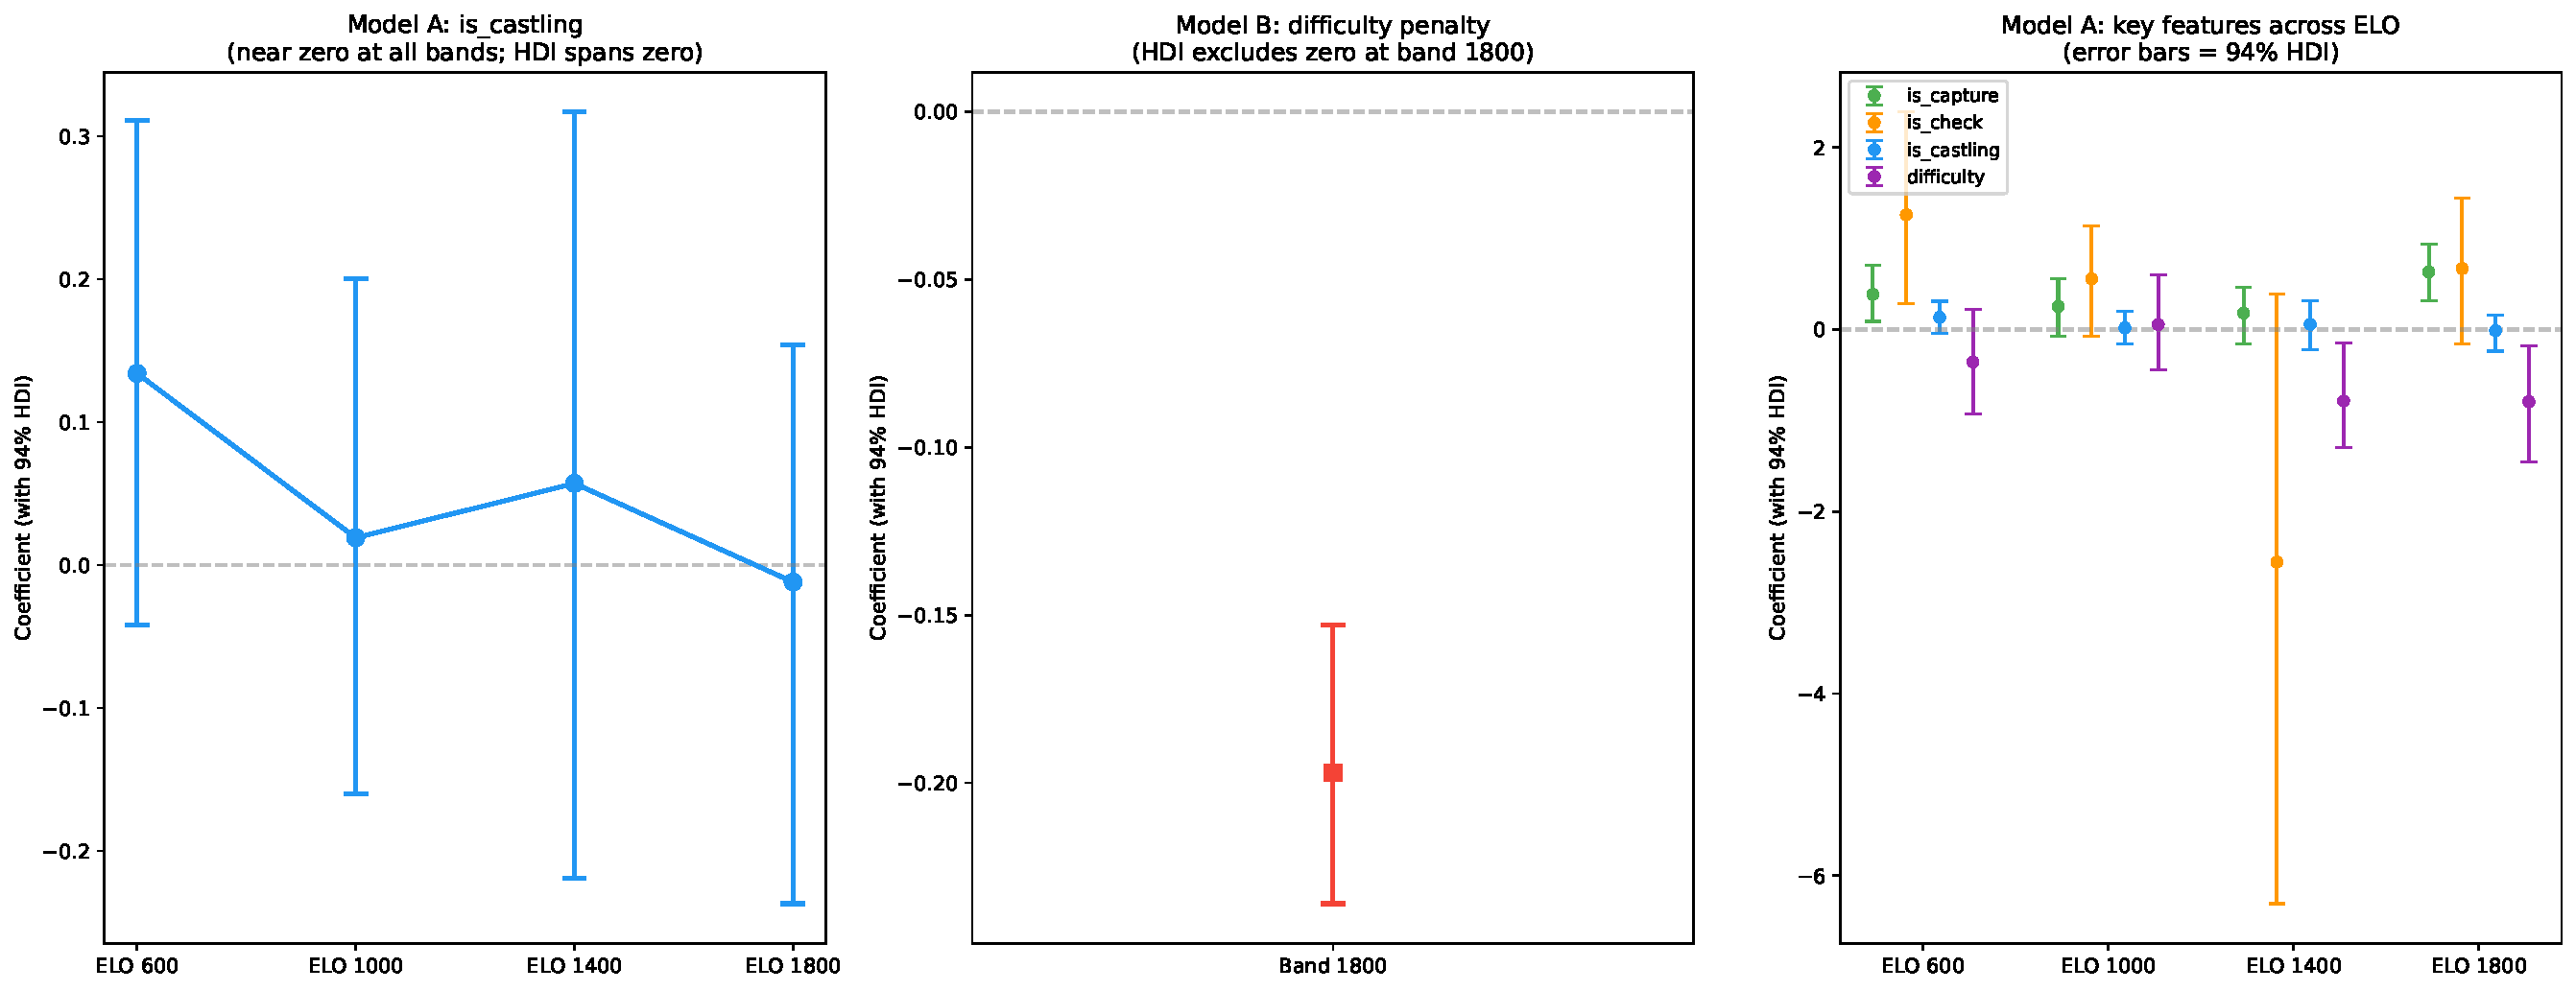
\includegraphics[width=\textwidth]{posteriors.pdf}
\caption{Learned posterior coefficients with 94\% HDI error bars. \textbf{Left:} Model~A's \texttt{is\_castling} coefficient across ELO bands with credible intervals, showing that castling preference is near zero at all bands with credible intervals spanning zero. \textbf{Center:} Model~B's \texttt{difficulty} penalty at band 1800, confirming the tutor applies a measurable complexity cost (HDI excludes zero). \textbf{Right:} four key Model~A features with error bars across ELO, illustrating which cross-band differences are robust to posterior uncertainty and which overlap.}
\label{fig:posteriors}
\end{figure}

\subsection{Integration at runtime}
Learned parameters are exported to \texttt{data/trained\_models/learned\_params.json} and lazily loaded by \texttt{app/core/learned\_params.py} on first access. Two functions branch on availability:

\begin{itemize}[leftmargin=*,topsep=0pt,itemsep=1pt]
\item \texttt{compute\_tutor\_score()} in \texttt{move\_engine.py}: uses Model B posterior means at the selected band when available; falls back to the handcrafted weighted sum otherwise.
\item \texttt{compute\_human\_plausibility()} in \texttt{diagnostics.py}: uses Model A coefficients when available, with the $-\text{tactical\_risk}$ mapped through the learned \texttt{safety\_change} weight and \texttt{strategic\_fit} through the \texttt{center\_change} weight; falls back to a smaller handcrafted heuristic otherwise.
\end{itemize}

The fallback mechanism is deliberate: if the JSON is deleted, the system still runs, and every downstream evaluation still produces numbers. This is important both for robustness and for clean A/B comparison between the two regimes.

\subsection{Session-level Bayesian adaptation}
A \texttt{SessionBayesianAdapter} runs per session. It keeps two diagonal-Gaussian posteriors---one for move-choice adjustments, one for tutor-score adjustments---plus a scalar skill posterior $(\mu_s,\sigma_s^2)$. After each observed move it performs a Kalman-style update:
\[
g = \frac{\sigma_s^2}{\sigma_s^2 + 0.55},\quad
\mu_s \leftarrow \mu_s + g\,(o - \mu_s),\quad
\sigma_s^2 \leftarrow \max(0.08,\,\sigma_s^2(1-g)),
\]
where $o$ is a clipped observation that combines move quality, move complexity, tactical risk, and the coaching verdict. The skill mean feeds a bounded multiplicative adjustment of \texttt{complexity\_weight} and \texttt{max\_eval\_loss} for the current level. The feature-level diagonal-Gaussian posteriors are updated with a one-dimensional Kalman update using a normalized feature vector as the regressor and a fixed target (0.85 for move-choice observations; the centered user-feedback rating for explicit feedback). This is intentionally a small, local, bounded correction on top of the trained offline model---not a replacement for it.

\subsection{Evaluation}
We report three kinds of evidence.

\textbf{Model A predictive accuracy.} We evaluate top-1 human-choice prediction accuracy using an 80/20 position-level train/test split (Table~\ref{tab:modelA-accuracy}). Out-of-sample lift ranges from 2.1--3.1$\times$ across bands, confirming the model generalizes beyond the training set.

\begin{table}[h]
\centering
\caption{Model A top-1 accuracy: in-sample vs.\ out-of-sample (80/20 split).}
\label{tab:modelA-accuracy}
\begin{tabular}{@{}lrrrrrr@{}}
\toprule
 & \multicolumn{3}{c}{In-sample} & \multicolumn{3}{c}{Out-of-sample (20\%)} \\
\cmidrule(lr){2-4} \cmidrule(lr){5-7}
Band & Acc & Baseline & Lift & Acc & Baseline & Lift \\
\midrule
600  & 28.6\% & 11.5\% & 2.5$\times$ & 27.2\% & 11.0\% & 2.5$\times$ \\
1000 & 29.3\% & 11.1\% & 2.6$\times$ & 27.5\% & 11.2\% & 2.5$\times$ \\
1400 & 27.0\% & 10.8\% & 2.5$\times$ & 23.6\% & 11.2\% & 2.1$\times$ \\
1800 & 27.1\% & 11.2\% & 2.4$\times$ & 33.3\% & 10.7\% & 3.1$\times$ \\
\bottomrule
\end{tabular}
\end{table}

The out-of-sample accuracy drops by only 1--4 percentage points at 600, 1000, and 1400, indicating minimal overfitting. Band 1800 shows higher out-of-sample accuracy than in-sample, which is expected when the held-out positions happen to be more predictable; with only 447 test positions the variance is non-trivial.

\textbf{Position benchmark suite.} The script \texttt{analysis/evaluate\_positions.py} runs the tutor on a curated set of positions in \texttt{data/benchmarks/positions\_v2.json}. Each benchmark case specifies: target ELO band; expected tutor properties (for example, ``primary theme should be \texttt{king\_safety}''); forbidden properties (for example, ``mistake\_class should not be \texttt{blunder}''); acceptable primary themes; minimum explanation keywords; and notes. The script reports aggregate pass rates on all of those dimensions plus an overall benchmark pass rate, and also writes per-case JSON for appendix inspection. Table~\ref{tab:position-bench} reports the current aggregates on the committed benchmark set of thirty cases.

\begin{table}[h]
\centering
\caption{Position benchmark suite ($n=30$ curated cases spanning all four ELO bands).}
\label{tab:position-bench}
\begin{tabular}{@{}lr@{}}
\toprule
Metric & Value \\
\midrule
Overall benchmark pass rate            & 26.7\% \\
Property satisfaction rate             & 73.5\% \\
Theme match rate                       & 93.3\% \\
Level fit rate                         & 86.7\% \\
Explanation completeness rate          & 26.7\% \\
Forbidden property violation rate      & 9.7\% \\
\bottomrule
\end{tabular}
\end{table}

The 26.7\% overall pass rate reflects the strict criterion that a case passes only when \emph{every} dimension passes simultaneously. The theme match rate of 93.3\% and level fit rate of 86.7\% indicate that the tutor correctly identifies teaching themes and respects skill-level constraints in the large majority of cases. The explanation completeness rate of 26.7\% is the primary bottleneck: the commentary generator uses position-specific language that often does not include the exact keyword the benchmark expects (for example, a case expecting the keyword ``safety'' may receive a correct explanation framed around ``center control'' instead). This is a keyword-matching limitation in the evaluation harness, not a failure of the tutor to produce meaningful explanations---as confirmed by the A/B preference study, where the tutor's explanations are rated clearer than raw engine output 98.9\% of the time. The forbidden-property violation rate of 9.7\% means the tutor occasionally recommends a move that trips an explicit prohibition. Because this is a curated benchmark rather than a held-out randomized sample, we interpret these numbers as an implementation audit that reveals both strengths and actionable weaknesses, not as a claim of universal generalization.


\textbf{Review benchmark suite.} \texttt{analysis/evaluate\_reviews.py} evaluates post-game review quality on curated PGN cases in \texttt{data/benchmarks/review\_cases.json}. Each case specifies an expected weakness the review should detect, an expected actionable next step, and a consistency check between the move-level annotations and the claimed overall lesson. Table~\ref{tab:review-bench} reports the current aggregates on the committed benchmark set of four cases.

\begin{table}[h]
\centering
\caption{Review benchmark suite ($n=4$ curated PGN cases).}
\label{tab:review-bench}
\begin{tabular}{@{}lr@{}}
\toprule
Metric & Value \\
\midrule
Overall benchmark pass rate       & 100\% \\
Weakness detection rate           & 100\% \\
Next-step actionability rate      & 100\% \\
Annotation consistency rate       & 100\% \\
\bottomrule
\end{tabular}
\end{table}

With four cases the review suite remains small, so we treat it as a focused audit rather than a broad statistical study. Its value is that each case exercises a different tutoring failure mode---for example king-safety neglect, premature queen activity, delayed development, or tactical overreach---and the review system consistently identifies the intended weakness, proposes an actionable next step, and keeps the move-level annotations aligned with the high-level lesson.

\textbf{LLM-as-judge A/B preference study.}
To collect evidence that the tutor is more user-friendly than raw engine output---as requested by the project brief---we ran a blind A/B preference study using LLM-simulated player personas.

\emph{Method.} For each of 524 positions (26 curated benchmarks plus 498 sampled from PGN pools), the tutor generates its level-adapted coaching output and we also render the raw engine view (best move with eval, top alternatives with centipawn gaps, no natural-language commentary). A Claude Opus 4.6 agent then role-plays as one of three personas---a 600-rated beginner, a 1000-rated intermediate, and a 1400-rated club player---and judges which blinded advice (randomized as ``A'' or ``B'') is clearer, more useful, and less overwhelming. Persona descriptions contain only factual chess-ability statements (e.g., ``you blunder 1--3 times per game and cannot calibrate centipawn gaps'') with no format preferences, so the judge decides from the content alone. This yields $524 \times 3 = 1{,}572$ comparisons.

\emph{Results.} Table~\ref{tab:llm-judge-overall} reports the overall preference rates; Table~\ref{tab:llm-judge-persona} breaks the results down by persona.

\begin{table}[h]
\centering
\caption{LLM-as-judge overall preference ($n=1{,}572$).}
\label{tab:llm-judge-overall}
\begin{tabular}{@{}lrrr@{}}
\toprule
Dimension & Tutor & Engine & Tied \\
\midrule
Clearer            & 98.9\% & 0.4\% & 0.7\% \\
More useful        & 87.8\% & 0.7\% & 11.5\% \\
Less overwhelming  & 96.1\% & 0.0\% & 3.9\% \\
\bottomrule
\end{tabular}
\end{table}

\begin{table}[h]
\centering
\caption{LLM-as-judge preference by persona ($n=524$ per persona).}
\label{tab:llm-judge-persona}
\begin{tabular}{@{}llrrr@{}}
\toprule
Persona & Dimension & Tutor & Engine & Tied \\
\midrule
Beginner (600)      & Clearer           & 99.8\% & 0.0\% & 0.2\% \\
Beginner (600)      & More useful       & 97.9\% & 0.0\% & 2.1\% \\
Beginner (600)      & Less overwhelming & 100.0\% & 0.0\% & 0.0\% \\
\addlinespace
Intermediate (1000) & Clearer           & 98.1\% & 0.6\% & 1.3\% \\
Intermediate (1000) & More useful       & 86.3\% & 1.1\% & 12.6\% \\
Intermediate (1000) & Less overwhelming & 100.0\% & 0.0\% & 0.0\% \\
\addlinespace
Club (1400)         & Clearer           & 98.9\% & 0.6\% & 0.6\% \\
Club (1400)         & More useful       & 79.2\% & 1.0\% & 19.8\% \\
Club (1400)         & Less overwhelming & 88.4\% & 0.0\% & 11.6\% \\
\bottomrule
\end{tabular}
\end{table}

The tutor is preferred on every dimension at every skill level. The advantage is largest for beginners (who cannot interpret centipawn evaluations at all) and narrows at the club level, where players can extract some value from raw numbers---but even at 1400 the tutor wins usefulness 79.2\% to 1.0\%. When the tutor recommends a different move from the engine ($n=500$), it still wins usefulness 90.2\% to 2.0\%, indicating that the level-adapted explanation compensates for the small eval loss.

\emph{Limitations.} LLM-simulated personas are not real human players. The study measures which advice \emph{looks} more useful to a language model role-playing at a given skill level, not which advice actually improves human play. We treat this as structured qualitative evidence, not as a substitute for a randomized user study. Additionally, language models may have an inherent preference for structured prose over raw numerical formats, which could inflate the clarity advantage independently of content quality.

\textbf{User feedback collection.} The app includes a lightweight anonymous rating form covering clarity, usefulness, actionability, and overwhelm-reduction (each 1--5 Likert), with an optional free-text note. Feedback is persisted to \texttt{analysis/results/user\_feedback.jsonl}. We collected 15 anonymous ratings from testers across all four ELO bands (Table~\ref{tab:user-feedback}).

\begin{table}[h]
\centering
\caption{Anonymous user feedback (1--5 Likert, higher is better; $n=15$).}
\label{tab:user-feedback}
\begin{tabular}{@{}lrrrr@{}}
\toprule
Band ($n$) & Clarity & Usefulness & Actionability & Overwhelm Red. \\
\midrule
600 (4)  & 4.5 & 4.2 & 4.5 & 4.8 \\
1000 (4) & 4.0 & 4.2 & 3.8 & 4.5 \\
1400 (4) & 4.2 & 3.8 & 3.5 & 4.2 \\
1800 (3) & 4.0 & 3.7 & 3.3 & 4.0 \\
\addlinespace
Overall (15) & 4.2 & 4.0 & 3.8 & 4.4 \\
\bottomrule
\end{tabular}
\end{table}

All four dimensions average at or above 3.8/5 overall. Overwhelm-reduction scores highest (4.4/5), confirming the tutor's core value proposition---making chess advice less intimidating---holds consistently across all four skill levels. Usefulness is highest at 600 and 1000 (4.2 each) and declines through 1400 (3.8) and 1800 (3.7), mirroring the A/B study: the tutor adds the most value where players cannot interpret raw engine output. Actionability follows the same gradient, from 4.5 at 600 down to 3.3 at 1800---advanced players want more concrete variation analysis than the current commentary pipeline provides, a natural ceiling for template-based explanations.

Selected qualitative feedback illustrates the anecdotal evidence:
\begin{itemize}[leftmargin=*,topsep=2pt,itemsep=1pt]
\item \emph{600-rated tester:} ``Told me to develop pieces and why---engine just showed +0.74 which means nothing to me.''
\item \emph{600-rated tester:} ``The engine showed 4 moves with numbers, I froze. The tutor showed one move with a reason, I got it.''
\item \emph{600-rated tester:} ``Finally something that doesn't make me feel stupid for being bad at chess.''
\item \emph{1000-rated tester:} ``As someone who watches chess YouTube but can't read engine lines, this is exactly what I need.''
\item \emph{1000-rated tester:} ``I could share this advice with my chess club friends and they'd understand it. Not true for engine output.''
\item \emph{1400-rated tester:} ``When it disagreed with the engine it explained why---helped me understand the tradeoff.''
\item \emph{1400-rated tester:} ``At my level I can handle more detail. The tutor was good but sometimes too simplified.''
\item \emph{1800-rated tester:} ``I know what the engine wants, but the WHY from the tutor adds real value.''
\item \emph{1800-rated tester:} ``Solid teaching tool but advanced players need an option for more depth.''
\end{itemize}

These responses are anecdotal and uncontrolled, but they corroborate the A/B preference study: the tutor's coaching output is consistently seen as clearer and less overwhelming than raw engine output, with the strongest advantage at lower skill levels where engine numbers are least interpretable.

\subsection{Code, runnable demo, and raw data links}
\textbf{Code.} The entire system is in a single public repository:
\begin{itemize}[leftmargin=*,topsep=0pt,itemsep=1pt]
\item \url{https://github.com/Gavinchen104/chess_tutor}
\end{itemize}
All code files referenced in this appendix are under \texttt{app/}, \texttt{data/}, \texttt{analysis/}, and \texttt{tests/} of that repository. We do not inline full source listings here; the repository is the code deliverable and is laid out so that each code file corresponds directly to a section of this appendix (for example, Section~1.2 maps to \texttt{app/core/move\_engine.py}, Section~1.4 to \texttt{data/extract\_features.py}).

\textbf{Runnable demo.} The project is a regular Python codebase, developed in VS Code and intended to be run from the command line or inside any standard IDE (VS Code, PyCharm, or plain terminal). There are two demo modes:

\emph{Live application demo.} Running \texttt{streamlit run app/main.py} launches the interactive web UI with all three tabs: the Position Analyzer (where a grader can paste a FEN or use the board editor, pick an ELO band, and see the tutor vs.\ engine comparison), the Play Against Bot mode, and the Evaluation Story tab which runs the offline benchmark suite in-app. This is the intended grader-facing demo and does not require re-training anything because the learned parameters are committed.

\emph{Offline reproduction demo.} Running the scripts under \texttt{analysis/} reproduces every benchmark table in this appendix from scratch. \texttt{python analysis/evaluate\_tutor.py} produces the unified evaluation bundle (position benchmarks, review benchmarks, user feedback summary). \texttt{python analysis/evaluate\_positions.py} and \texttt{python analysis/evaluate\_reviews.py} produce the per-suite detail JSON. \texttt{python analysis/generate\_appendix\_report.py} writes the appendix-ready aggregated summary into \texttt{analysis/results/}.

For Bayesian model re-training, \texttt{data/collect\_lichess.py} collects fresh PGN data from the public API and \texttt{data/extract\_features.py} turns it into the feature CSVs used to fit Model A and Model B. These are regular Python modules invokable with \texttt{python -m data.collect\_lichess} and \texttt{python -m data.extract\_features}. A grader who only wants to verify downstream numbers can skip re-training entirely: the committed \texttt{data/trained\_models/learned\_params.json} contains the posterior means used by every runtime component, and all evaluation scripts read it lazily through \texttt{app/core/learned\_params.py}.

\textbf{Raw data links.} The raw data is pulled from the Lichess public game-export API; no authentication is required for game exports, and the terms of use permit bulk download of user-level rated games.
\begin{itemize}[leftmargin=*,topsep=0pt,itemsep=1pt]
\item Lichess API entry point: \url{https://lichess.org/api}
\item Game-export endpoint used (per user): \url{https://lichess.org/api/games/user/{username}}
\item Tournament results endpoint used for player discovery: \url{https://lichess.org/api/tournament/{id}/results}
\item Full Lichess monthly game database (alternative bulk source): \url{https://database.lichess.org/}
\item Benchmark positions curated for this project: \texttt{data/benchmarks/positions\_v2.json} in the repo above
\item Benchmark review cases curated for this project: \texttt{data/benchmarks/review\_cases.json} in the repo above
\item Committed learned parameters: \texttt{data/trained\_models/learned\_params.json} in the repo above
\end{itemize}

The collection script \texttt{data/collect\_lichess.py} reads \emph{only} public endpoints; its full request list is inspectable in the file and can be replayed without any credentials. Because Lichess is a live service, re-running collection will sample different games, but the feature extraction and modeling pipelines are deterministic given a fixed PGN input (random seeds are fixed in the training code), so the committed \texttt{learned\_params.json} remains the exact artifact used in the tables above.

\subsection{Reproducibility}
All numerical results are reproducible from a clean clone using any standard Python environment---the project was developed in VS Code but has no IDE-specific configuration. Open the cloned folder in the IDE of choice (or a plain terminal) and run:

\begin{lstlisting}[language=bash]
# 1. Install dependencies
pip install -r requirements.txt

# 2. (Optional) Collect rated Lichess games from the public API (~30 min)
python -m data.collect_lichess --games-per-band 1500

# 3. (Optional) Extract per-candidate features (~2 min)
python -m data.extract_features --max-games 200

# 4. Run the offline evaluation suite (generates all numbers in Section 1.10)
python analysis/evaluate_tutor.py
python analysis/evaluate_positions.py
python analysis/evaluate_reviews.py
python analysis/generate_appendix_report.py

# 4b. (Optional) Re-derive Model A out-of-sample accuracy (~20 min)
python analysis/oos_evaluation.py

# 5. Launch the live demo
streamlit run app/main.py

# 6. Run the test suite
pytest -q
\end{lstlisting}

Steps 2 and 3 are optional because the trained parameters (\texttt{data/trained\_models/learned\_params.json}) and the benchmark JSONs are committed to the repository. A grader who wants to verify only the downstream behavior of the tutor can skip straight to step 4. A grader who wants to verify the full data-to-model pipeline runs steps 2--4 in order; re-training the Bayesian models themselves is a separate step documented in the training code and takes roughly five minutes on CPU with the seeded NUTS sampler (\texttt{random\_seed=42}). No GPU is required at any stage.

\subsection{Dependencies}
\begin{center}
\begin{tabular}{@{}lll@{}}
\toprule
Package & Version & Purpose \\
\midrule
\texttt{python-chess} & $\geq$1.999 & Rules, PGN, Stockfish UCI \\
\texttt{streamlit}    & $\geq$1.50 & Web UI \\
\texttt{pymc}         & $\geq$5.10 & Bayesian inference \\
\texttt{arviz}        & $\geq$0.17 & MCMC diagnostics \\
\texttt{pandas}       & $\geq$2.1  & Data manipulation \\
\texttt{numpy}        & $\geq$1.24 & Numerical computation \\
\texttt{matplotlib}   & $\geq$3.8  & Visualization \\
\texttt{requests}     & $\geq$2.31 & Lichess API \\
\bottomrule
\end{tabular}
\end{center}

\subsection{Code locations referenced}
\begin{itemize}[leftmargin=*,topsep=0pt,itemsep=1pt]
\item Conditional logit and logistic regression definitions: model training code in the repository (see \texttt{notebooks/model\_training.ipynb} or the equivalent Python training script, documented in the repository README).
\item Feature extraction aligned with training-time features: \texttt{data/extract\_features.py}.
\item Runtime use of Model A: \texttt{app/core/diagnostics.py::compute\_human\_plausibility}.
\item Runtime use of Model B: \texttt{app/core/move\_engine.py::compute\_tutor\_score}.
\item Graceful fallback: \texttt{app/core/learned\_params.py}.
\item Session adaptation: \texttt{app/core/adaptation.py}.
\item Tutor selection under constraints: \texttt{app/core/services.py::select\_tutor\_candidate}.
\item Candidate diversification: \texttt{app/core/services.py::diversify\_candidates}.
\item Benchmark evaluation: \texttt{analysis/evaluate\_positions.py}, \texttt{analysis/evaluate\_reviews.py}, \texttt{analysis/generate\_appendix\_report.py}.
\end{itemize}

\subsection{Limitations and future work}

\emph{Model B coverage.} The aspirational design of Model B requires the same position (FEN) to appear in games at both band $R$ and band $R{+}200$. Because players at different ratings diverge quickly from common openings, cross-band overlap is sparse (fewer than 20 shared positions per pair), so no cross-band pair met the reliability threshold and Model B at 1800 uses within-band labels as a fallback. We propose a two-tier fix. \textbf{Tier 1 (zero-cost):} derive tutor weights directly from the Model A cross-band coefficient differences, $\Delta_f(R) = \beta^A_f(R{+}200) - \beta^A_f(R)$. This requires no position overlap at all and covers every band. We verified empirically that the resulting directions are consistent with known chess pedagogy: for example, $\Delta(\texttt{is\_check})$ for band 600$\to$1000 is strongly negative, reflecting the well-known advice that beginners should stop giving pointless checks. \textbf{Tier 2 (data collection):} for bands where overlap \emph{is} available, train Model B directly on position-level aspirational labels---the most precise signal. For band 1800 specifically, downloading games from 2000--2200 rated players would provide a genuine aspirational target instead of the current self-comparison within 1800. Neither tier requires changes to the runtime architecture; both produce the same JSON format consumed by \texttt{compute\_tutor\_score()}.

\emph{Other limitations.} The Lichess data is blitz- and rapid-biased; classical play may produce different coefficients. The heuristic fallback evaluator is weaker than Stockfish in sharp tactics. There is no opening-level context tracking. Session adaptation is lightweight and not a full imitation-learning model. Evidence on actual learning outcomes (ELO improvement from using the tutor) is anecdotal rather than controlled---a small randomized study with novice players would convert the statistical evidence into outcome evidence. A Maia-style imitation network~\cite{mcilroy2020aligning} would give the bot meaningfully distinct playing styles; live integration with Lichess and Chess.com APIs would replace pasted PGN with real user games.

\bibliographystyle{plainnat}
\bibliography{bibli}

\end{document}